\documentclass[crop,tikz]{standalone}

\usetikzlibrary{calc,positioning,shapes}

\begin{document}
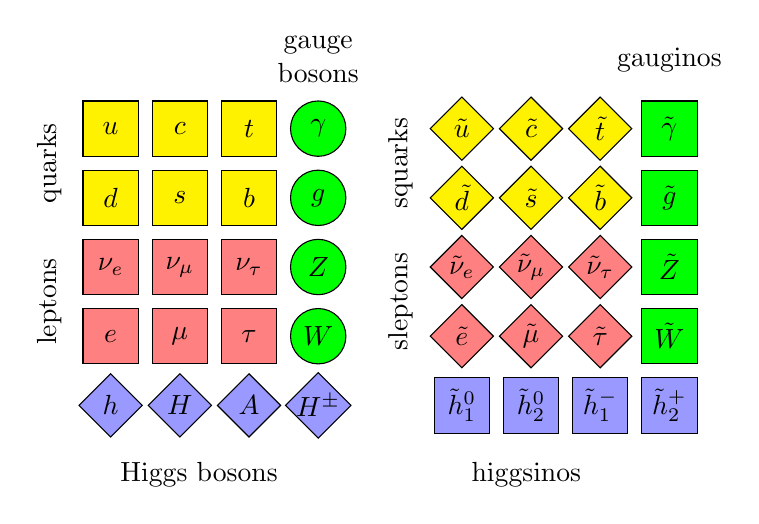
\begin{tikzpicture}[
  node distance   = 2.5em,
  quark/.style    = {rectangle, black, draw, fill=yellow , minimum width=2em  , text centered, minimum height=2em  , inner sep=0pt},
  lepton/.style   = {rectangle, black, draw, fill=red!50 , minimum width=2em  , text centered, minimum height=2em  , inner sep=0pt},
  gauge/.style    = {circle   , black, draw, fill=green  , minimum size=2em   , text centered, minimum height=2em  , inner sep=0pt},
  scalar/.style   = {diamond  , black, draw, fill=blue!40, minimum width=2.3em, text centered, minimum height=2.3em, inner sep=0pt},
  squark/.style   = {diamond  , black, draw, fill=yellow , minimum width=2.3em, text centered, minimum height=2.3em, inner sep=0pt},
  slepton/.style  = {diamond  , black, draw, fill=red!50 , minimum width=2.3em, text centered, minimum height=2.3em, inner sep=0pt},
  gaugino/.style  = {rectangle, black, draw, fill=green  , minimum size=2em   , text centered, minimum height=2em  , inner sep=0pt},
  higgsino/.style = {rectangle, black, draw, fill=blue!40, minimum width=2em  , text centered, minimum height=2em  , inner sep=0pt},
  ]
  % standard model fields
  \node[quark] (u) {$u$};
  \node[quark, below of=u] (d) {$d$};
  \node[quark, right of=u] (c) {$c$};
  \node[quark, below of=c] (s) {$s$};
  \node[quark, right of=c] (t) {$t$};
  \node[quark, below of=t] (b) {$b$};
  \node[lepton, below of=d] (nue) {$\nu_e$};
  \node[lepton, below of=nue] (e) {$e$};
  \node[lepton, right of=nue] (numu) {$\nu_\mu$};
  \node[lepton, below of=numu] (mu) {$\mu$};
  \node[lepton, right of=numu] (nutau) {$\nu_\tau$};
  \node[lepton, below of=nutau] (tau) {$\tau$};
  \node[gauge, right of=t] (gamma) {$\gamma$};
  \node[gauge, below of=gamma] (gluon) {$g$};
  \node[gauge, below of=gluon] (Z) {$Z$};
  \node[gauge, below of=Z] (W) {$W$};
  \node[scalar, below of=e] (h) {$h$};
  \node[scalar, below of=mu] (H) {$H$};
  \node[scalar, below of=tau] (A) {$A$};
  \node[scalar, below of=W] (Hpm) {$H^\pm$};
  % labels
  \node[rotate=90,above] (quarks)  at ($(u)!0.5!(d)+(-0.5,0)$)  {quarks};
  \node[rotate=90,above] (leptons) at ($(nue)!0.5!(e)+(-0.5,0)$) {leptons};
  \node[below of=h, anchor=west] (higgs) {Higgs bosons};
  \node[above of=gamma, align=center] (gauge) {gauge\\ bosons};
  % supersymmetric partners
  \node[squark, right=3em of gamma] (su) {$\tilde{u}$};
  \node[squark, below of=su] (sd) {$\tilde{d}$};
  \node[squark, right of=su] (sc) {$\tilde{c}$};
  \node[squark, below of=sc] (ss) {$\tilde{s}$};
  \node[squark, right of=sc] (st) {$\tilde{t}$};
  \node[squark, below of=st] (sb) {$\tilde{b}$};
  \node[slepton, below of=sd] (snue) {$\tilde{\nu}_e$};
  \node[slepton, below of=snue] (se) {$\tilde{e}$};
  \node[slepton, right of=snue] (snumu) {$\tilde{\nu}_\mu$};
  \node[slepton, below of=snumu] (smu) {$\tilde{\mu}$};
  \node[slepton, right of=snumu] (snutau) {$\tilde{\nu}_\tau$};
  \node[slepton, below of=snutau] (stau) {$\tilde{\tau}$};
  \node[gaugino, right of=st] (sgamma) {$\tilde{\gamma}$};
  \node[gaugino, below of=sgamma] (sgluon) {$\tilde{g}$};
  \node[gaugino, below of=sgluon] (sZ) {$\tilde{Z}$};
  \node[gaugino, below of=sZ] (sW) {$\tilde{W}$};
  \node[higgsino, below of=se] (sh) {$\tilde{h}_1^0$};
  \node[higgsino, below of=smu] (sH) {$\tilde{h}_2^0$};
  \node[higgsino, below of=stau] (sA) {$\tilde{h}^-_1$};
  \node[higgsino, below of=sW] (sHpm) {$\tilde{h}^+_2$};
  % labels
  \node[rotate=90,above] (squarks)  at ($(su)!0.5!(sd)+(-0.5,0)$)  {squarks};
  \node[rotate=90,above] (sleptons) at ($(snue)!0.5!(se)+(-0.5,0)$) {sleptons};
  \node[below of=sh, anchor=west] (shiggs) {higgsinos};
  \node[above of=sgamma, align=center] (sgauge) {gauginos};
\end{tikzpicture}
\end{document}
